\subsubsection{概要}
たまチームは、ROS 2に移行されたemcl2パッケージ
emcl2\_ros2を用いて、
屋外でロボットに自律走行させた。
目標に関しては、つくばチャレンジ初参加のチームメンバーであることも考え、
無理に完走を目指さず、交差点手前までのナビゲーションということにした。

\subsubsection{使用したハードウェアとソフトウェア}

たまチームのシステムの構成を図\ref{fig:tama_system_diagram}に示す.
ロボットに搭載された2D LiDARとIMUから、
Raspberry Pi 4B+を介し、センサ情報をノートPCに送信する。
ノートPCでは自己位置推定、経路計画が行われ、
その結果として得られた制御指令がRaspberry Pi 4に返される。
マッピングにはslam\_toolboxを利用し、
経路計画にはNav2を利用した。
%また、自己位置推定においては、
%昨年度まで利用されていたemcl2パッケージを
%ROS 2に移行した、emcl2\_ros2利用している。

\begin{figure}[h]
  \begin{center}
    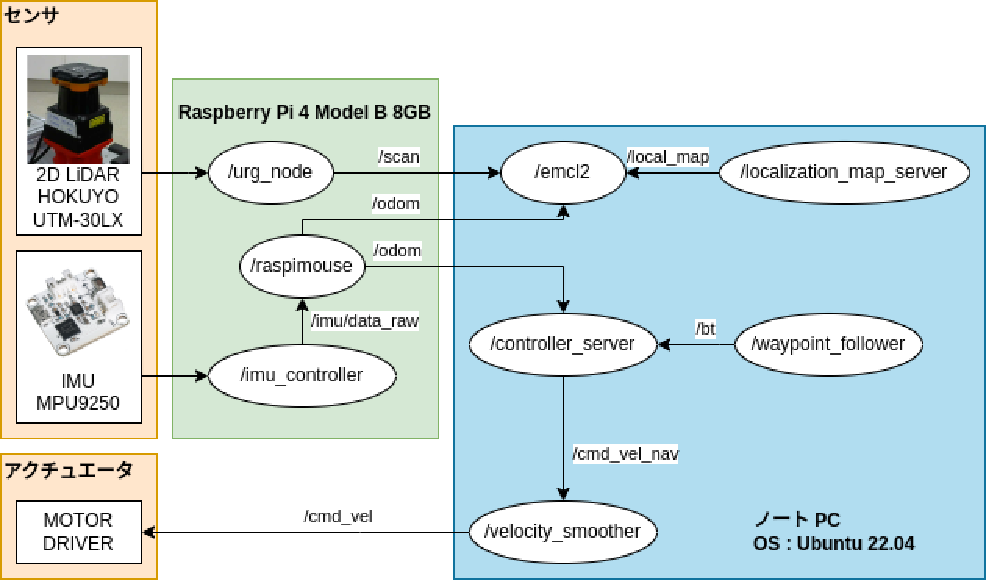
\includegraphics[width=1.0\linewidth]{figs/tama_system_diagram.pdf}
    \caption{たまチームのシステム構成}
    \label{fig:tama_system_diagram}
  \end{center}
\end{figure}